\documentclass[conference]{IEEEtran}
\usepackage{graphicx}
\begin{document}
\title{Comparing CNN Architectures on CIFAR-10}
\author{\IEEEauthorblockN{Sample Student}\IEEEauthorblockA{Department of Computer Science}}
\maketitle
\begin{abstract}
This report compares two convolutional neural networks for image classification. The final classifier
architecture, the effective learning rate schedule and the official training split are described below.
\end{abstract}
\section{Introduction}
Image classification remains a standard benchmark for convolutional architectures. We study how
quickly two well-known networks converge and how their final performance differs across datasets,
following the usual practice of reporting validation curves and test results side by side.
\section{Experimental Setup}
Each model was trained for 20 epochs with a batch size of 128 on a single GPU. We used a weight decay of $5\times10^{-4}$ and a learning rate of $10^{-3}$. Data augmentation used random crops and horizontal flips, which is the
conventional configuration for this benchmark and keeps the comparison fair across architectures.
\section{Results}
Fig.~\ref{fig:acc} shows the validation accuracy and Fig.~\ref{fig:loss} the training loss.
\begin{figure}[t]\centering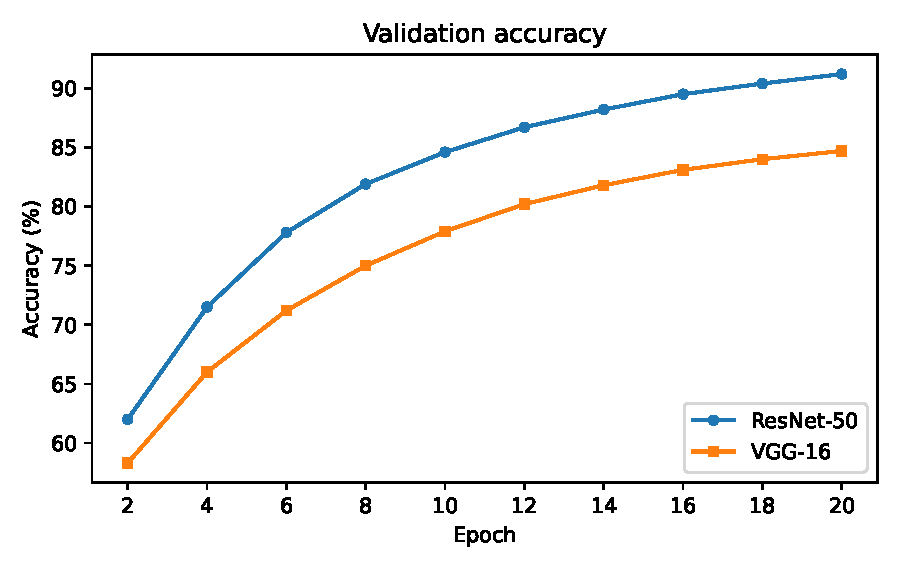
\includegraphics[width=\columnwidth]{fig_acc.pdf}
\caption{Validation accuracy of ResNet-50 and VGG-16 during training.}\label{fig:acc}\end{figure}
ResNet-50 reached 91.2\% validation accuracy at epoch 20 (Fig. 1). VGG-16 achieved 88.0\% validation accuracy at epoch 20. At epoch 10, VGG-16 is 6.7 points lower than ResNet-50. The difference between the two architectures is substantial and consistent
throughout training, which suggests that the residual connections help optimisation considerably.
\begin{figure}[t]\centering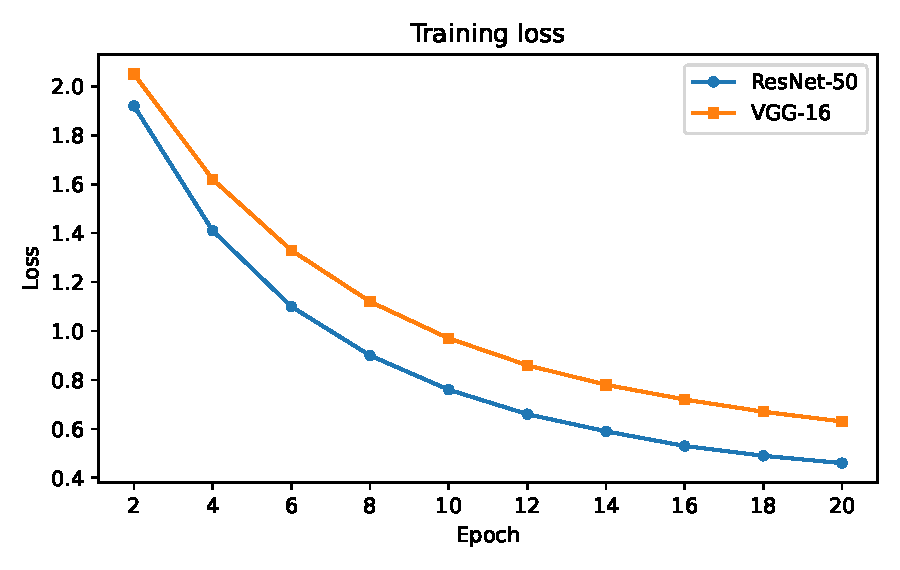
\includegraphics[width=\columnwidth]{fig_loss.pdf}
\caption{Training loss of both models.}\label{fig:loss}\end{figure}
From epoch 2 to epoch 20, the training loss of ResNet-50 decreased by 76\%. The training loss of VGG-16 was 0.63 at epoch 20. The training loss of ResNet-50 was 0.30 at epoch 20. The training loss of ResNet-50 is $4.6\times10^{-1}$ at epoch 20.
\begin{figure}[t]\centering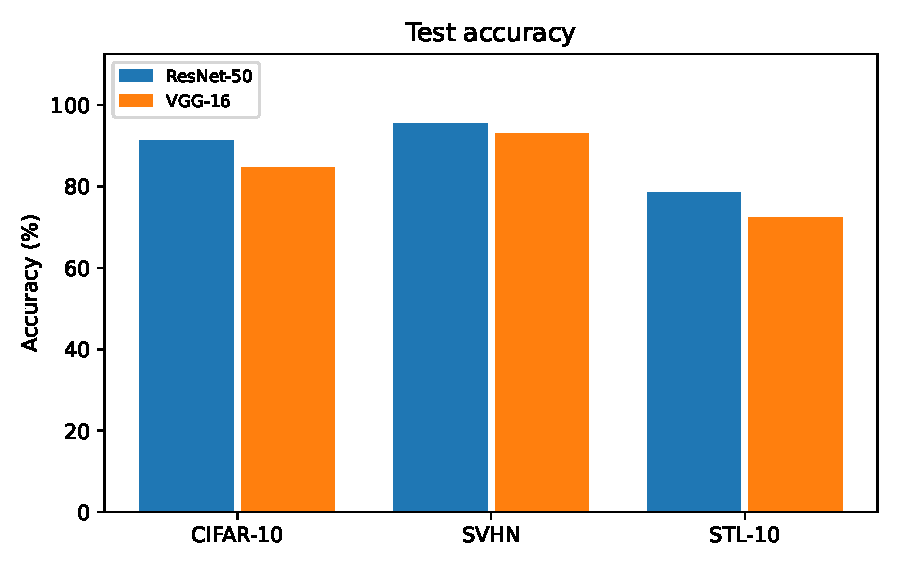
\includegraphics[width=\columnwidth]{fig_test.pdf}
\caption{Test accuracy on three datasets.}\label{fig:test}\end{figure}
On SVHN, ResNet-50 achieves 95.4\% test accuracy (Fig. 3). On STL-10, ResNet-50 is 2.1 points better than VGG-16. VGG-16 reaches eighty-four point seven percent validation accuracy at epoch twenty.
\section{Conclusion}
Residual networks train faster and generalise better on every dataset considered here. Further
experiments with stronger regularisation are left for future work.
\end{document}
